\documentclass{../grid-link-report}
\SetClassAssetsDir{../class-assets}

\newcommand{\projectassetsdir}{../project-assets}

\project{Heywood BESS}
\client{Atmos}
\title{Releasable User Guide - PSSE}
\docnumber{HEYWOODBESS-GR-RPT-001}
\issueddate{25 July 2025}
\revision{1-1-0}
\revisionhistorycsvpath{report-assets/revision-history.csv}
\clientlogopath{\projectassetsdir/client-logo.jpg}

\usepackage{listings}
\usepackage{tabto}
\usepackage[justification=centering]{caption}%
\usepackage{pgfplotstable} % For reading and displaying tables from CSV files
\usepackage{booktabs}      % For better-looking tables
\usepackage{adjustbox}
\usepackage{float}

\begin{document}
	% Draft commands
	%\adddraftstamp
	%s\listoftodos
	
	\frontmatter
	\maketitle
	
	\makedisclaimer
	\clearpage
	\tableofcontents
	\makerevisionhistorypage
	%\makeaboutgridlink
	
	\mainmatter
	
	\chapter{Introduction}
	\section{Project Overview}
    The Heywood Battery Energy Storage System (HEYWOODBESS) is a $\pm~285MW/1140MWh$ Battery Energy Storage Project, is located 5 km from the town of Heywood and 300 km west of Melbourne in Victoria as shown in Figure~\ref{fig:project-location}. The project is expected to connect directly to the existing 275 kV Heywood terminal station via a single high voltage cable.

HEYWOODBESS will include 92 SMA Sunny Central 4.6 MVA (SCS 4600 UP-S) converters which will be connected to two 275/33/33kV, 160MVA three winding transformers through a 33kV reticulation system. Each converter will have a dedicated 33/0.69kV, 4.6 MVA step up transformer.


\begin{figure}[H]
	\centering
	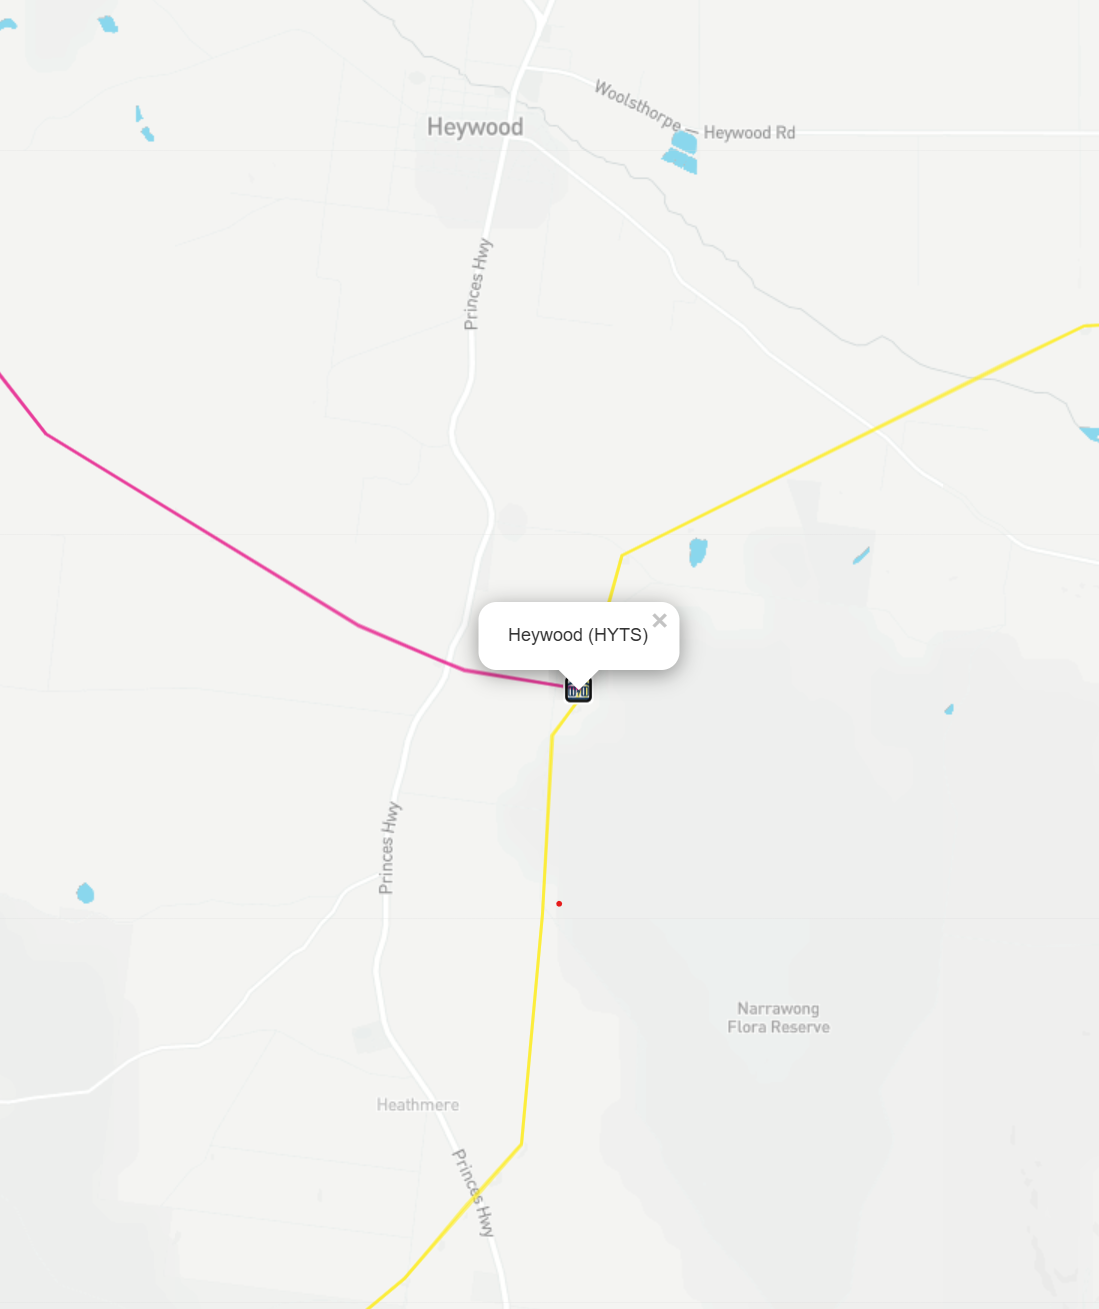
\includegraphics[width=0.7\textwidth]{\projectassetsdir/project-location.png} % Change example-image-a to the filename of your image
	\caption{Project location}
	\label{fig:project-location}
\end{figure}


    
    Project information is given as Table \ref{tab:projectinformation}.
    
    % Project information	
    {	
    	\thicktablelines
    	\begin{longtable}{|>{\columncolor{gray!20}}C{7cm}|C{8cm}|}
    		\caption{Project Information}
    		\label{tab:projectinformation} \\
    		\toprule
    		
    		\rowcolor{tableheaderblue}
    		\bfseries \color{white}Feature & \bfseries \color{white}Description \\
    		\endhead
    		\bottomrule \endfoot
    		\csvreader[
    		separator=semicolon,
    		late after line=\\\hline,
    		late after last line=,
    		before reading={\catcode`\#=12},
    		after reading={\catcode`\#=6}]%
    		{report-assets/poc-data.csv}{1=\CSVItem,2=\CSVComment}{\CSVItem & \CSVComment}
    	\end{longtable}
    	
    }
    

	\chapter{Model Overview}
	
	\section{PSSE load flow model description}

	The PSSE model is an aggregated representation of the \ac{BESS}. Four aggregated generator machine, including an aggregated converter transformer from 33 / 0.69 kV are connected to the LV sides of two 275 / 33 / 33 kV grid transformers via lumped impedances representing the reticulation network. The equivalent impedance of the 33 kV reticulation network is calculated based on a detailed model of the reticulation network which accommodates all 92 4.6 MVA converters.
	
	Tables \ref{tab:aggr-plant} - \ref{tab:line-cables-inv} summaries the details on the aggregated plant and equipment models. The following equipment are included in the load flow model of the plant:
	
	\begin{itemize}
		\item 4 X lumped generator representing project converters. 
		\item 4 x lumped two-winding MV 33/0.69 kV converter transformers
		\item 4 x aggregated MV reticulation representing the lumped impedance from converter transformers to 33kv switchboard  (modelled as X,R,B quantities)
		\item 4 x aggregated MV reticulation representing the lumped impedance from 33kV switchboard to grid transformers (modelled as X,R,B quantities)		 
		\item 2 x 275 / 33 / 33 kV grid transformers

		\item 1 x 275 kV underground cable between grid transformer and connection point (POC)		
	\end{itemize}


	The connection point of HEYWOODBESS is located 1.4 km away from the 275 kV side of the main grid transformer, connected via a 275 kV underground cable. Additional items are included in the PSSE model to represent the external grid, and allow for adequate testing of the model to be carried out. The below list summarises these items.
	
	\begin{itemize}
		\item 1 x generator at 275 kV infinite bus representing external grid. 
		\item 1 x 275 kV dummy line (impedance variable to represent various grid strength conditions)
		\item 1 x zero impedance dummy line at 275 kV (measurement purposes only)
		\item 1 x zero impedance 275 / 275 kV transformer (for phase angle shifting testing).  
	\end{itemize}
	
	The PSSE single line diagram of the single machine infinite bus load flow model for the HEYWOODBESS is shown in the below Figure \ref{fig:psse-model-sld}.
	
	\begin{figure}[H]
		\centering
		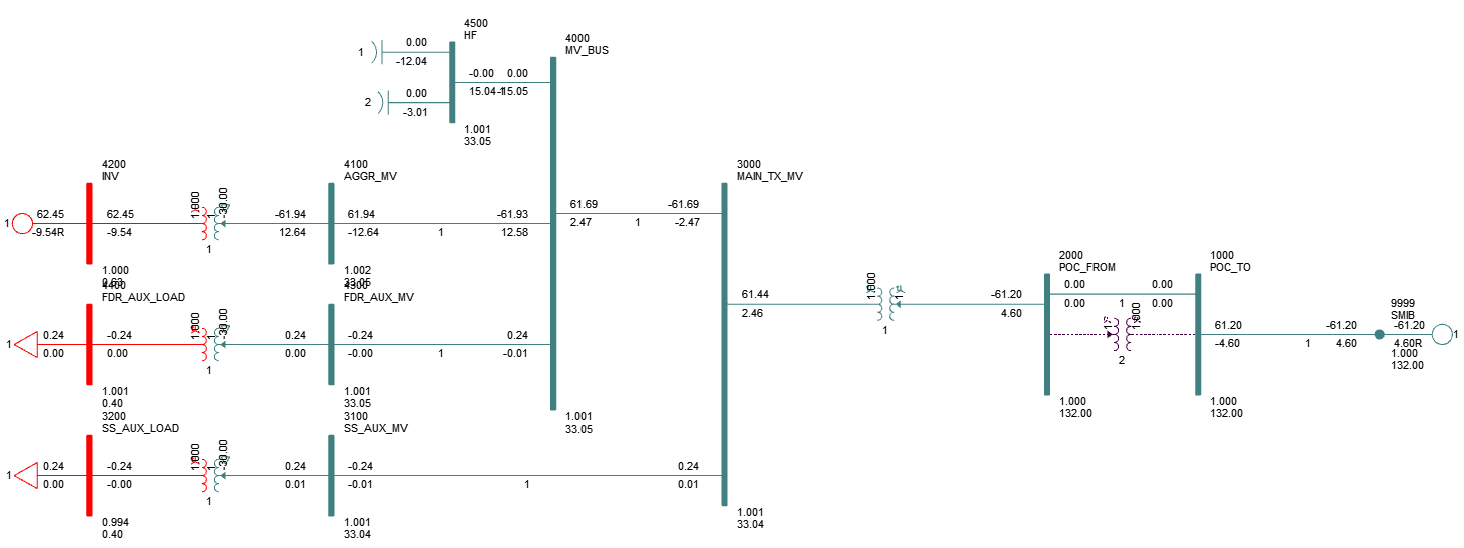
\includegraphics[width=0.9\textwidth]{\projectassetsdir/PSSEsld.png}
		\caption{PSSE load flow model SLD}
		\label{fig:psse-model-sld}
	\end{figure}

	The rated capability of the generator load flow model is shown in Table \ref{tab:aggr-plant}. Transformer parameters are shown in Table \ref{tab:aggr-transformer} and Table \ref{tab:inv-transformer}. Lines parameters are shown in Table \ref{tab:line-cables-275kV} - \ref{tab:line-cables-inv}. This model was prepared under the system strength conditions shown in Table \ref{tab:fault-details}.
	
	It should be noted that the generator load flow capability is based on rated data rather than the expected capability of the plant under steady state conditions. Active power flow at the generator point of connection should be restricted to \pm285 MW, and reactive power should be restricted to limits of \pm112.575 MVAr \footnote{The machine must be dispatched so as to not exceed the limits at the POC} under steady state conditions. The maximum generator active power \footnote{The maximum active power and reactive power must not exceed Mbase limitations;$\sqrt{P_{\text{gen}}^2 + Q_{\text{gen}}^2} \leq M_{\text{base}}$ } and reactive power are given in Table \ref{tab:aggr-plant}.


	% Aggregate plant parameter table
	{%
		\thicktablelines
		\begin{longtable}{|C{3cm}|C{6cm}|C{2cm}|>{\centering\arraybackslash}m{4cm}|}
			\caption{Aggregated plant parameters}
			\label{tab:aggr-plant}
			\\	
			\toprule
			
			\rowcolor{tableheaderblue}
			\bfseries \color{white}Parameters & \bfseries \color{white}Description & \bfseries \color{white}Units & \bfseries \color{white}HEYWOODBESS \\
			\endhead
			\bottomrule \endfoot
			\csvreader[
			separator=comma,
			late after line=\\\hline,
			late after last line=,
			before reading={\catcode`\#=12},
			after reading={\catcode`\#=6}]%
			{report-assets/aggregate-plant-parameters.csv}{1=\CSVParameters,2=\CSVDescription,3=\CSVUnits, 4=\CSVHEYWOODBESS}{\CSVParameters & \CSVDescription & \CSVUnits & \CSVHEYWOODBESS}
			\\\hline
		\end{longtable}
	}

		
			% Aggregate transformer parameter table
		{%
		\thicktablelines
		\begin{longtable}{|C{6cm}|C{6cm}|} 
			\caption{Grid transformer parameters}
			\label{tab:aggr-transformer}
			\\	
			\toprule
			
			\rowcolor{tableheaderblue}
			\bfseries \color{white}Parameter & \bfseries \color{white}Value
			\endhead
			\bottomrule \endfoot
			\csvreader[
			separator=comma,
			late after line=\\\hline,
			late after last line=,
			before reading={\catcode`\#=12},
			after reading={\catcode`\#=6}]%
			{report-assets/GTX.csv}{1=\COLA,2=\COLB}{\COLA & \COLB}
			\\\hline
		\end{longtable}
	}

		{%
		\thicktablelines
		\begin{longtable}{|C{6cm}|C{6cm}|} 
			\caption{Inverter transformer parameters}
			\label{tab:inv-transformer}
			\\	
			\toprule
			
			\rowcolor{tableheaderblue}
			\bfseries \color{white}Parameter & \bfseries \color{white}Value
			\endhead
			\bottomrule \endfoot
			\csvreader[
			separator=comma,
			late after line=\\\hline,
			late after last line=,
			before reading={\catcode`\#=12},
			after reading={\catcode`\#=6}]%
			{report-assets/INVTX.csv}{1=\COLA,2=\COLB}{\COLA & \COLB}
			\\\hline
		\end{longtable}
	}
		% Lines and Cable parameters for Cable from HVTX to POC
	{%
		\thicktablelines
		\begin{longtable}{|C{2cm}|C{3cm}|C{6cm}|C{1cm}|C{4cm}|} 
			\caption{Lines and Cable parameters for Cable connecting from HV Transformer to POC (based on 100MVA and 275kV)}
			\label{tab:line-cables-275kV}
			\\	
			\toprule
			
			\rowcolor{tableheaderblue}
			\bfseries \color{white}CableGroup & \bfseries \color{white}Parameter & \bfseries \color{white}Description & \bfseries \color{white}Units & \bfseries \color{white}HEYWOODBESS \\
			\endhead
			\bottomrule \endfoot
			\csvreader[
			separator=comma,
			late after line=\\\hline,
			late after last line=,
			before reading={\catcode`\#=12},
			after reading={\catcode`\#=6}]%
			{report-assets/lines-cables-parameters-275kV.csv}{1=\CSVCableGroup,2=\CSVParameter,3=\CSVDescription,4=\CSVUnits,5=\CSVHEYWOODBESS}{\CSVCableGroup & \CSVParameter & \CSVDescription & \CSVUnits & \CSVHEYWOODBESS }
			\\\hline
		\end{longtable}
	}
	
	
	
	
	% Lines and Cable parameters for Cable connecting to Main Transformer
	{%
	\thicktablelines
	\begin{longtable}{|C{2cm}|C{3cm}|C{6cm}|C{1cm}|C{4cm}|} 
		\caption{Lines and Cable parameters for Cable connecting from 33kV switchboard to HV transformer (based on 100MVA and 33kV)}
		\label{tab:line-cables-inv}
		\\	
		\toprule
		
		\rowcolor{tableheaderblue}
		\bfseries \color{white}CableGroup & \bfseries \color{white}Parameter & \bfseries \color{white}Description & \bfseries \color{white}Units & \bfseries \color{white}HEYWOODBESS \\
		\endhead
		\bottomrule \endfoot
		\csvreader[
		separator=comma,
		late after line=\\\hline,
		late after last line=,
		before reading={\catcode`\#=12},
		after reading={\catcode`\#=6}]%
		{report-assets/lines-cables-parameters-MainTX.csv}{1=\CSVCableGroup,2=\CSVParameter,3=\CSVDescription,4=\CSVUnits,5=\CSVHEYWOODBESS}{\CSVCableGroup & \CSVParameter & \CSVDescription & \CSVUnits & \CSVHEYWOODBESS }
		\\\hline
	\end{longtable}
}
	
		% Lines and Cable parameters for Cable connecting from MVTX to 33kV switchboard
	{%
		\thicktablelines
		\begin{longtable}{|C{2cm}|C{3cm}|C{6cm}|C{1cm}|C{4cm}|} 
			\caption{Lines and Cable parameters for Cable connecting from MV transformers to 33kV switchboard (based on 100MVA and 33kV)}
			\label{tab:line-cables-inv}
			\\	
			\toprule
			
			\rowcolor{tableheaderblue}
			\bfseries \color{white}CableGroup & \bfseries \color{white}Parameter & \bfseries \color{white}Description & \bfseries \color{white}Units & \bfseries \color{white}HEYWOODBESS \\
			\endhead
			\bottomrule \endfoot
			\csvreader[
			separator=comma,
			late after line=\\\hline,
			late after last line=,
			before reading={\catcode`\#=12},
			after reading={\catcode`\#=6}]%
			{report-assets/lines-cables-parameters-Inv.csv}{1=\CSVCableGroup,2=\CSVParameter,3=\CSVDescription,4=\CSVUnits,5=\CSVHEYWOODBESS}{\CSVCableGroup & \CSVParameter & \CSVDescription & \CSVUnits & \CSVHEYWOODBESS }
			\\\hline
		\end{longtable}
	}

	%
	{	
		\thicktablelines
		\begin{longtable}{|C{5cm}|C{4cm}|C{2cm}|}
			\caption{System strength conditions}
			\label{tab:fault-details} \\
			\toprule
			\rowcolor{tableheaderblue}
			\bfseries \color{white}Condition & \bfseries \color{white}Fault Level (MVA) & \bfseries \color{white}X/R Ratio \\
			\endhead
			\bottomrule \endfoot
			\csvreader[
			late after line=\\\hline,
			late after last line=,
			before reading={\catcode`\#=12},
			after reading={\catcode`\#=6}]% 
			{report-assets/fault-details.csv}{1=\CSVParameter,2=\CSVValue,3=\CSVUnit}{\CSVParameter & \CSVValue & \CSVUnit}
			\\\hline
		\end{longtable}
	}	

	
	\chapter{Reactive Capability}
	The reactive capability curves for HEYWOODBESS at 35°C, 40°C and 50°C are shown in Figures \ref{fig:pq-curve-35degC}, \ref{fig:pq-curve-40degC} and \ref{fig:pq-curve-50degC}. The automatic access standard has been shown as a dotted line, and is defined by the upper corner points $P_{max}$=285 MW, $Q_{max}$=112.575 MVAr, $P_{max}$=285 MW, $Q_{min}$=-112.575 MVAr, and the lower corner points $P_{min}$=-285 MW, $Q_{min}$=-112.575 MVAr, $P_{min}$=-285 MW, $Q_{max}$=112.575 MVAr.
	
			
	\begin{figure}[H]
		\centering
		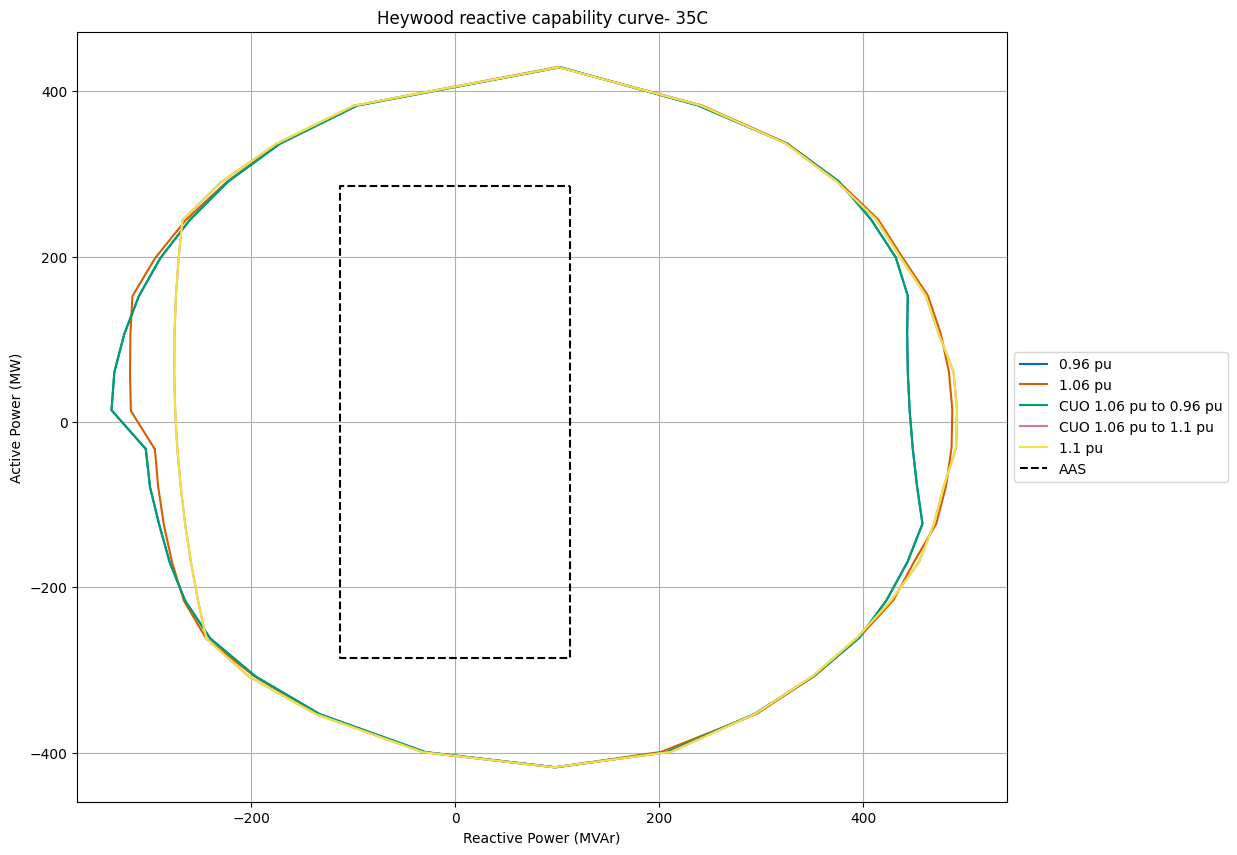
\includegraphics[width=0.8\textwidth]{\projectassetsdir/capability-curves/new_Heywood reactive capability curve- 35C.png}
		\caption{35°C Reactive capability curve for HEYWOODBESS}
		\label{fig:pq-curve-35degC}
	\end{figure}
	
	\begin{figure}[H]
		\centering
		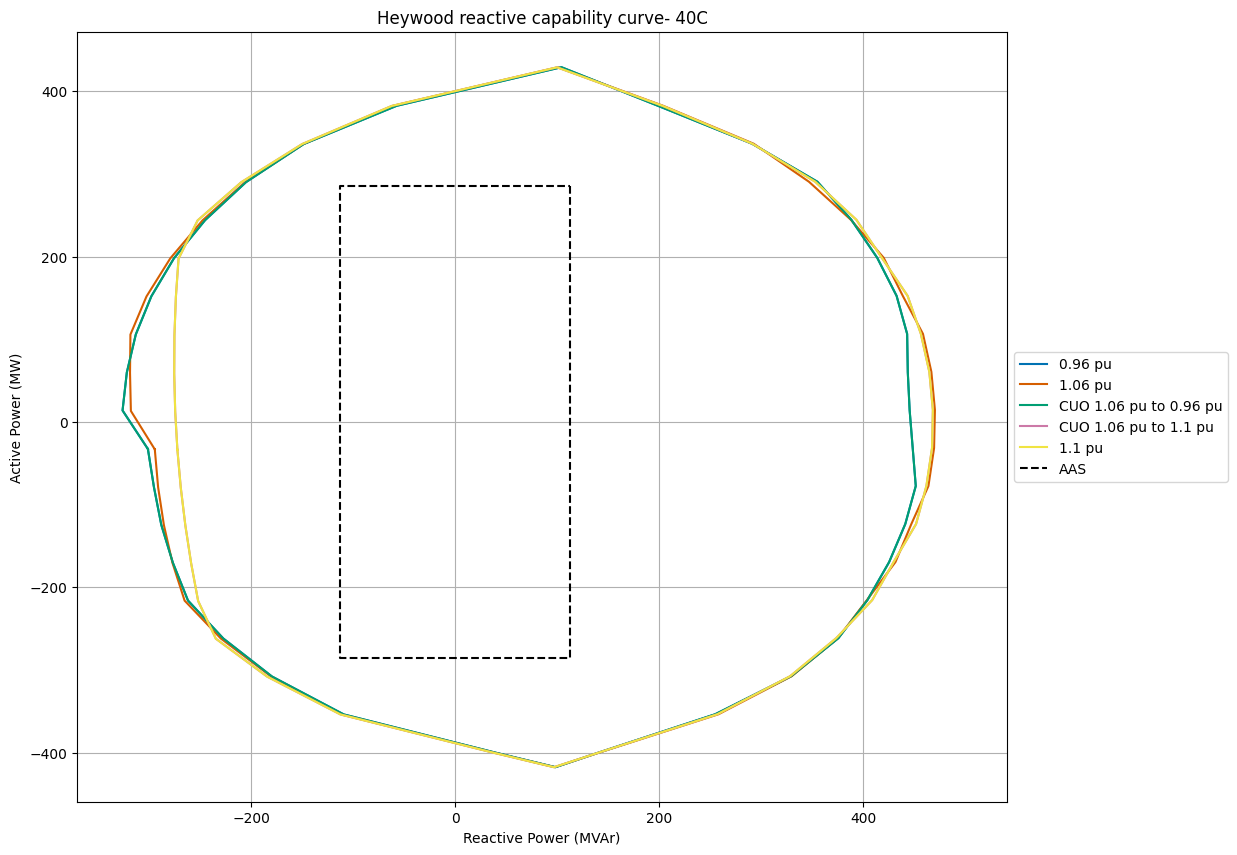
\includegraphics[width=0.8\textwidth]{\projectassetsdir/capability-curves/new_Heywood reactive capability curve- 40C.png}
		\caption{40°C Reactive capability curve for HEYWOODBESS}
		\label{fig:pq-curve-40degC}
	\end{figure}
	
	\begin{figure}[H]
		\centering
		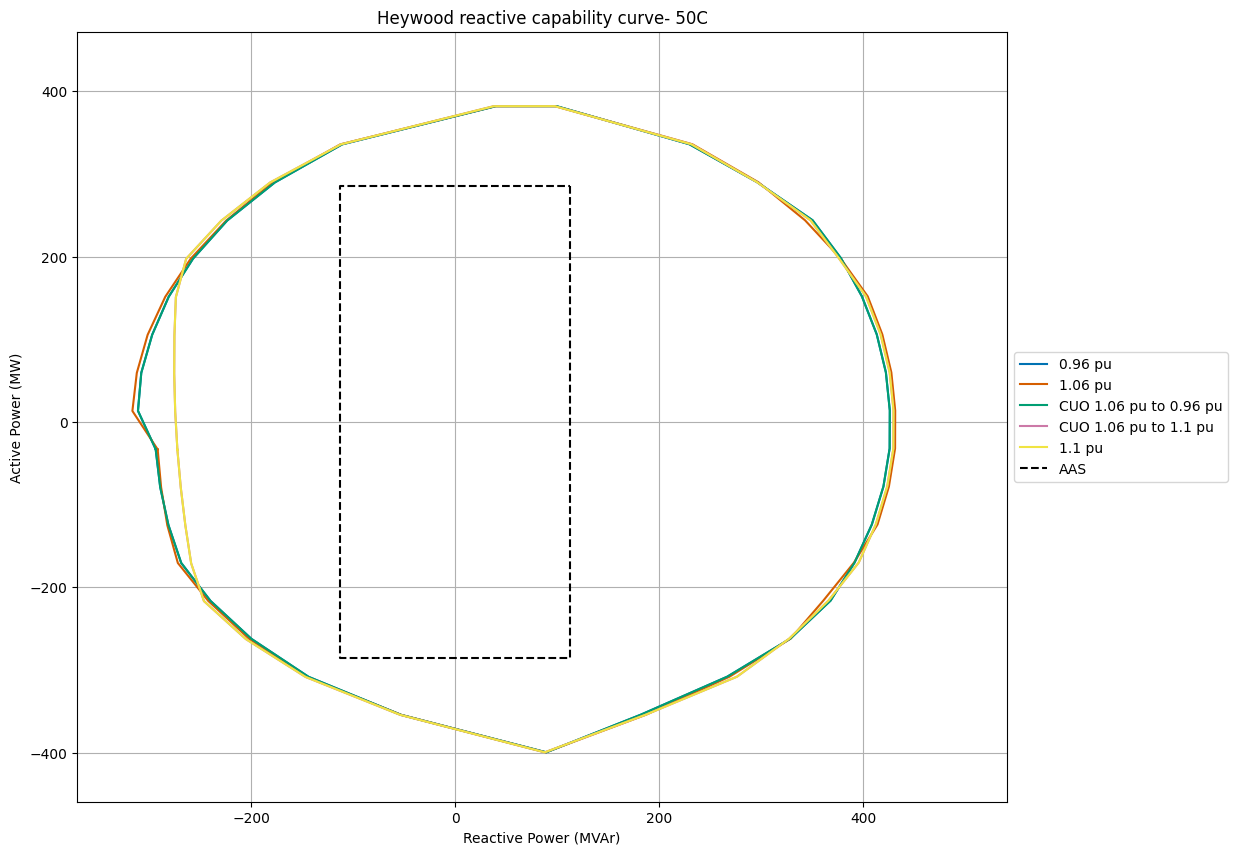
\includegraphics[width=0.8\textwidth]{\projectassetsdir/capability-curves/Heywood reactive capability curve- 50C.png}
		\caption{50°C Reactive capability curve for HEYWOODBESS}
		\label{fig:pq-curve-50degC}
	\end{figure}
	
	\chapter{Dynamic Model}
	
	\section{Overview}
	
	
	The PSSE plant model has six dynamic models that will control the response of the plant for dynamic RMS simulations in PSSE. These are:
	
	\begin{itemize}
		\item 4 x converter SMAGF308 models which control the response of the four lumped generator representing the plant converters, taking instructions from the \ac{PPC}.
		\item 1x PPC FLNCPPC_V1020 model which controls the aggregate response of the plant under "normal" operating conditions.
		\item 1x OLTC \ac{OLTC} model which assist to regulate the voltage at the LV side of the grid transformers.
	\end{itemize}
	
	SMAGF_G308_344_IVF150.dll and FLUENCE_v349_V1020_IVF150.dll dynamic link libary (dll) are included for the SMA models. The "FLUENCE_v349_V1020_IVF150.dll" file must be added for the PPC model to operate. The "SMAGF_G308_344_IVF150.dll" file must be added for the converter models to operate. The OLTC model is the default library model included in PSSE and does not require any external libraries to operate.

	
	The \ac{PPC}'s control loops prepare active and reactive power set points in per unit, which are then sent to each converter. Each converter then multiplies these per unit control values by their MVA rating to determine the MW and MVAr set points.
	
	\section{Initialisation}
	
	The HEYWOODBESS model is initialised from the solved load flow, with dynamic models taking their initial STATEs and VARs from these conditions.
	
	The dynamic plant model does not take inputs from default PSSE load flow limit parameters, i.e. Qmax, Qmin, Pmax, and Pmin. Users should therefore take care that the model is not initialised outside of its active and reactive power capability limits, despite this being possible to do so under load flow conditions. Initialising outside of these limits can result in D-state warnings, and will prevent the model from achieving a flat run. The model should normally be set to control voltage at its point of connection to 1.06, unless an alternative voltage control mode such as reactive power or power factor is activated, or this would result in the model initialising outside of a limit.
	

	
	\section{Plant control}
	This section will explain the default expected mode of operation of the plant, as well as how to operate the plant under alternative control modes if required, for both normal and abnormal operating conditions. Under normal conditions, the plant will seek to control active and reactive power at its point of connection, via reference signals passed from the power plant controller to the converters. The plant also has a seperate operating mode for fault / overvoltage conditions, where the PPC may temporarily freeze to allow the converters to operate under reactive current control. Details of the operating modes and interactions between plant are explained in the following sections.
	
	\subsection{Reactive Power Control Schemes}
	The Fluence PPC supports multiple reactive power control modes, selectable via the \textbf{RPCM} setting (ICON(M+5)). The default reactive power control mode is the remote voltage control mode with VSL droop control(ICON(M+5)=5) and the available modes and their configurations are summarised below:


	

	
	
	\subsubsection{RPCM = 5 — Remote Voltage Control Mode}

	When RPCM is set to 5, the system operates in remote voltage control mode with \ac{VSL} droop logic. In this mode, the reactive power output is determined based on the deviation of the measured remote bus voltage from a target voltage setpoint. In order to use this control mode the VSL is required to be always enabled. Key parameters to adjust reactive power control are shown below:

	\begin{itemize}
		\item ICON M+5 - must be set to 5 for the PPC to operate in remote voltage control mode
		\item ICON M+7 - must be set to 1 for enabling the VSL function
		\item VAR L+18 - can be adjusted to set the remote voltage setpoint Vset

	\end{itemize}
	
\subsubsection{Voltage Droop Characteristics}


Given the 4\% voltage droop characteristic of the Heywood BESS, the corresponding relationship is defined as follows:


\[
\text{Droop} =  \left[ \frac{\text{p.u.}}{\text{p.u.}} \right] = \frac{(U - U_{\text{set}})/U_n}{(Q - Q_{\text{set}})/Q_n} = \frac{U - U_{\text{set}}}{Q - Q_{\text{set}}} \cdot \frac{Q_n}{U_n}
\]
 (with Qn = 112.575 MVAr)



	
	
	\begin{figure}[H]
		\centering
		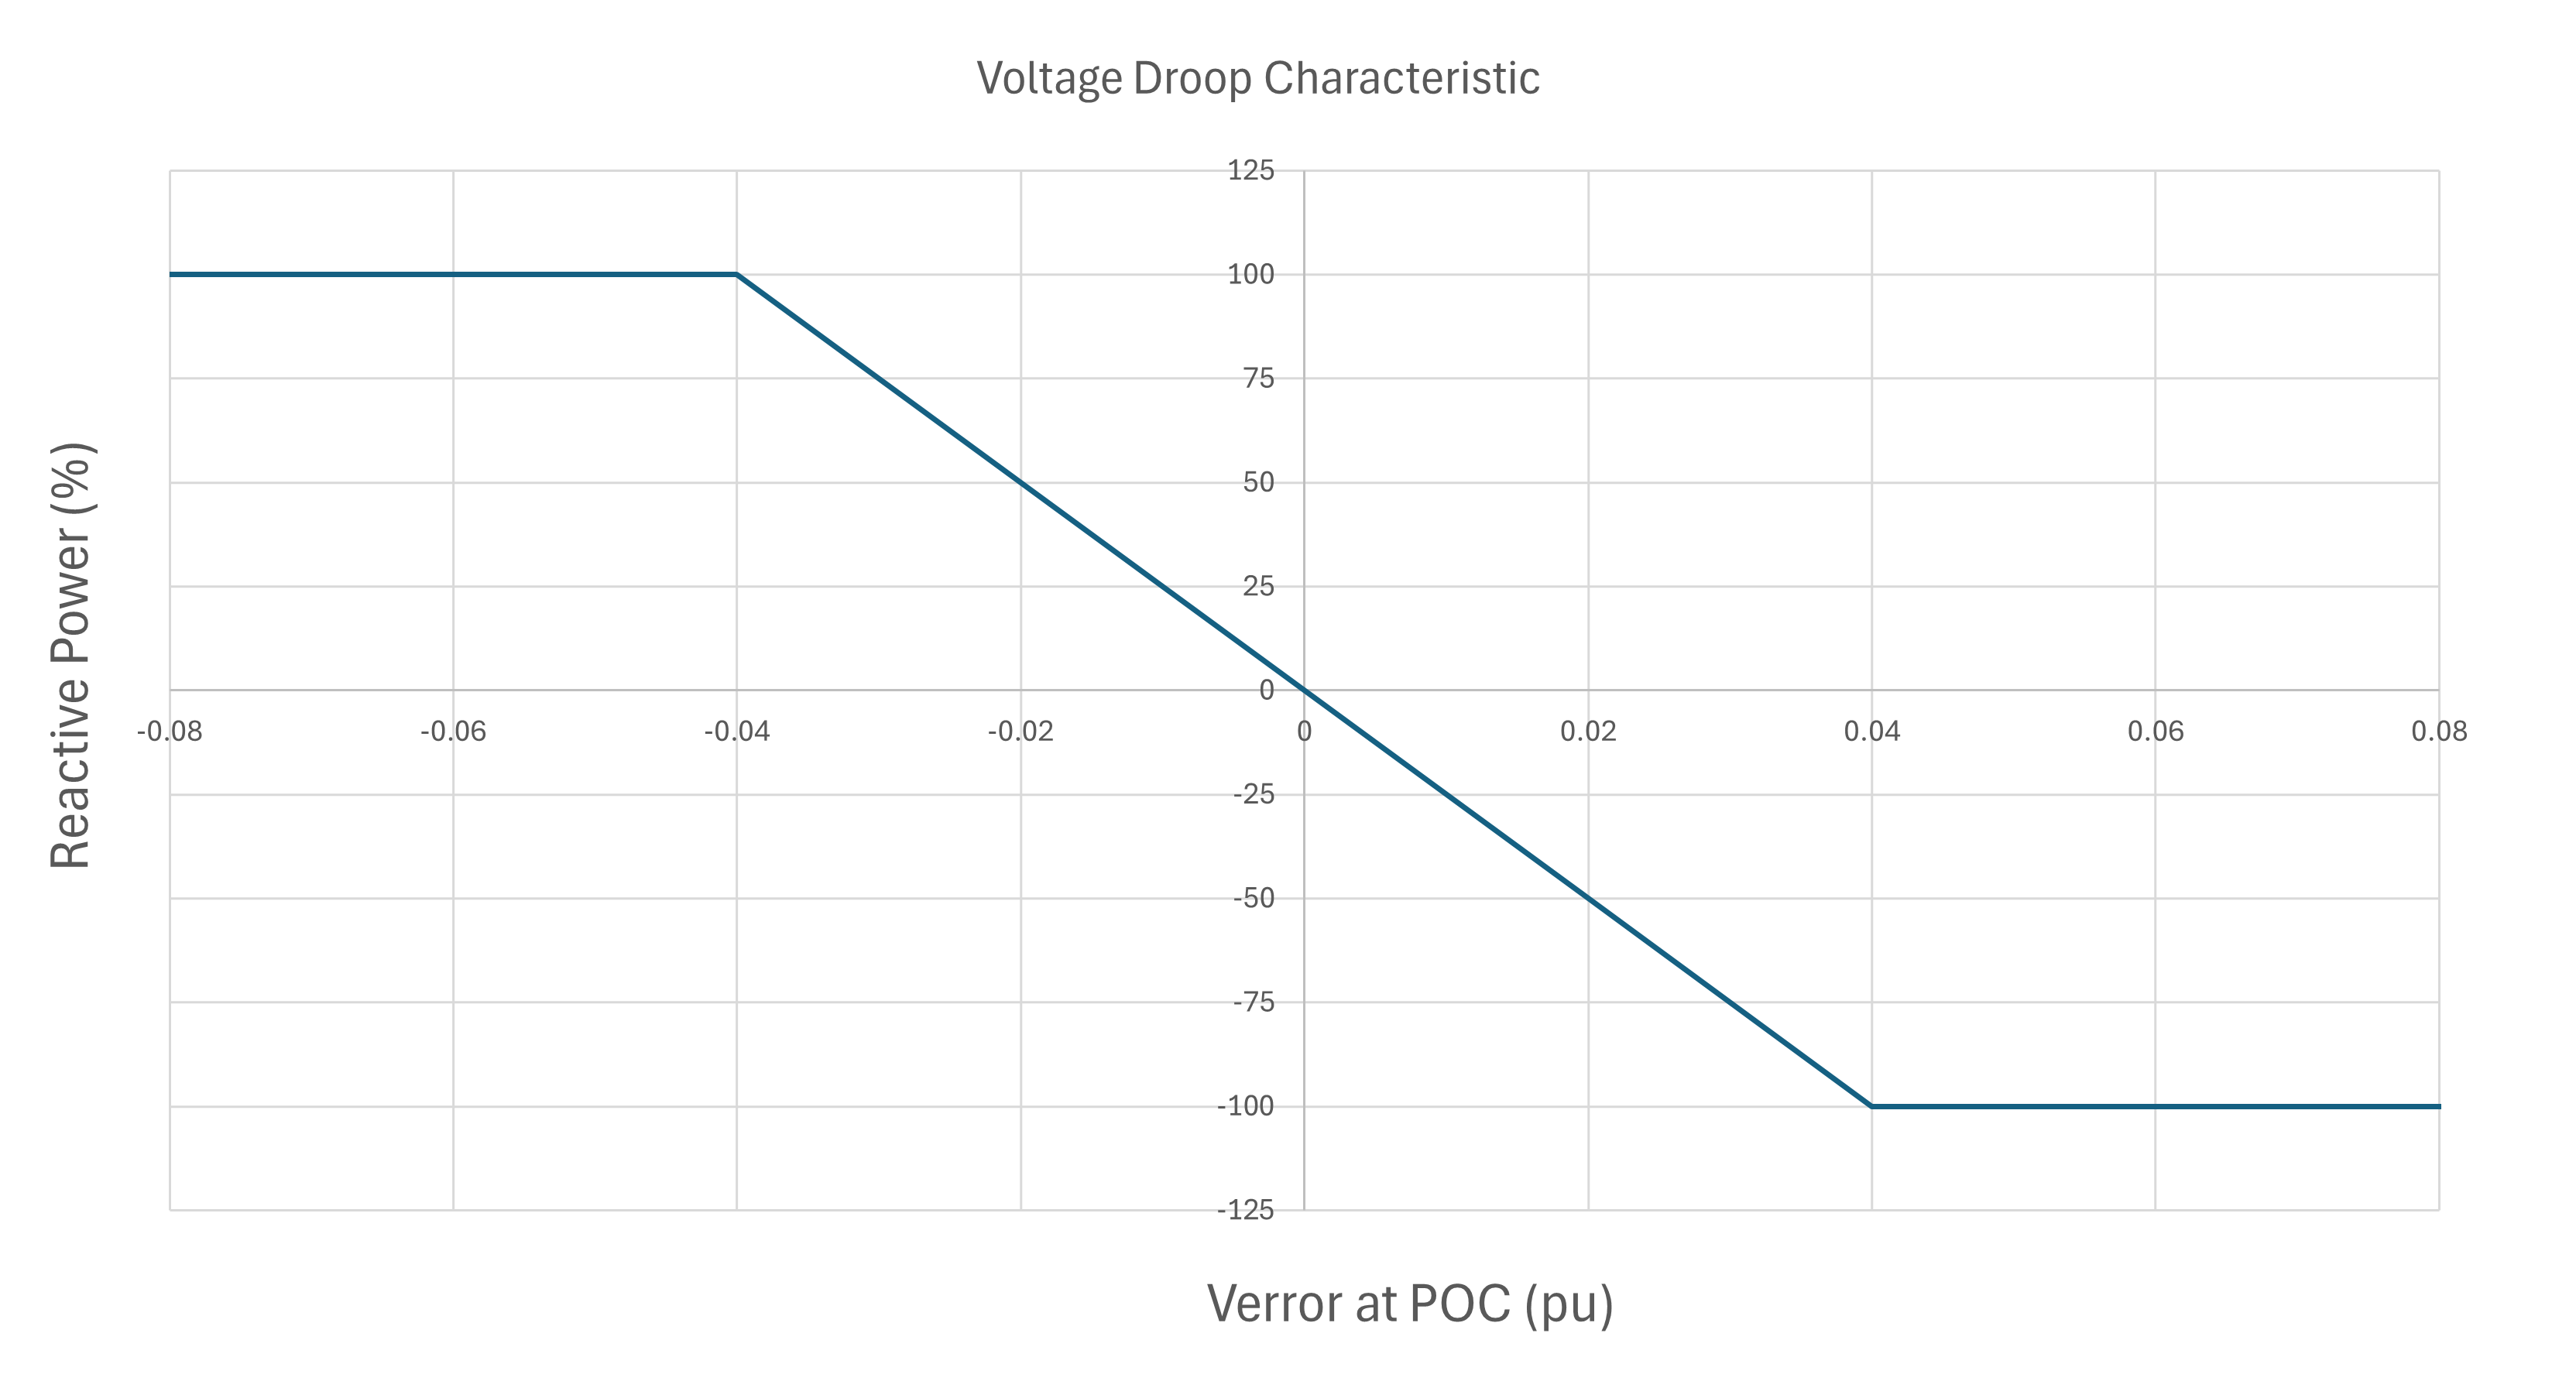
\includegraphics[width=0.9\textwidth]{report-assets/images/vdroop-char.png}
		\caption{Voltage droop characteristic}
		\label{fig:vdroop-char}
	\end{figure}
	
	\dansquicktable{|C{4cm}|C{4cm}|}
	{Voltage droop characteristic tabulated}
	{v-droop-char}
	{\bfseries \color{white}Voltage Error at POC (pu) & \bfseries \color{white}Reactive Power (MVAr)}
	{report-assets/v-droop-char-new.csv}
	
	\subsubsection{RPCM = 2 — Power Factor Control Mode}

	When RPCM is set to 2, the BESS operates in power factor control mode, Key parameters to adjust power factor control are shown below:
	
	\begin{itemize}
		\item ICON M+5 - must be set to 2 for the PPC to operate in power factor control mode
		\item VAR L+7 - can be adjusted to set power factor target at the POC
	\end{itemize} 
	
	\subsubsection{RPCM = 3 — Remote Reactive Power Control Mode}
	
	When RPCM is set to 3, the BESS enters remote reactive power control mode. In this mode, the reactive power at a specified remote branch is regulated based on a command signal (QRMTCMD, set via VAR(L+1)). Key parameters to adjust droop control are shown below:
	
	\begin{itemize}
		\item ICON M+5 - must be set to 3 for the PPC to operate in remote reactive power control mode
		\item ICON M+2 - can be adjusted to set the location of the controlled branch (Should not be changed under normal operation)
		\item VAR L+1 - can be adjusted to set the reactive power at a specified remote branch
	\end{itemize}

	
	
	\subsubsection{OLTC control}
	The \ac{OLTC} have been specified to regulate the voltage at the medium voltage side of the main transformers to be 1 p.u.

	The OLTC1 model, as a PSSE library model, takes inputs from the load flow parameters of their transformers. The Vmax(pu) and Vmin(pu) parameters are used to specify voltage regulation, with Rmax and Rmin defining range of regulation, and tap size defined by the formula $\frac{Rmax-Rmin}{tap positions}$.

	The transformer is set to operate with a time delay of 20 seconds and 7s mechanical operation time. These delays are adjustable by the model CONS J and J+2.	
			{
		\thicktablelines
		\begin{longtable}{|C{6cm}|C{4cm}|} 
			\caption{Grid transformer OLTC Details}
			\label{tab:main-transformer}
			\\	
			\toprule
			
			\rowcolor{tableheaderblue}
			\bfseries \color{white}Parameter & \bfseries \color{white}Value\\
			\endhead
			\bottomrule \endfoot
			\csvreader[
			separator=semicolon,
			late after line=\\\hline,
			late after last line=,
			before reading={\catcode`\#=12},
			after reading={\catcode`\#=6}]%
			{report-assets/main_transformer.csv}{1=\CSVParameter,2=\CSVValue}{\CSVParameter &\CSVValue}
			\\\hline
		\end{longtable}
	}
	
	\subsection{Active power and frequency control}
	
	The \ac{PPC} regulates active power output through setpoint commands to the converters to target a fixed active power setpoint at the point of connection. Under frequency disturbances, the plant operates under droop control and will diverge from its reference setpoint. The plant operates with a droop characteristic of 5.0\% on a 50 Hz base, and a frequency deadband of +/- 0.015 Hz. 
	
	The PPC can operate in both local active power control and remote active power control, to be defined by the user. The PPC operates in remote active power control mode by default. This characteristic is shown in Figure \ref{fig:fdroop-char}. 
	\subsubsection{PRCF = 1 — Local Active power Control Mode}
	
	Key parameters for local active power and frequency control are shown below: 
	
	\begin{itemize}
		\item ICON M+6 - must be set to 1 to enable local active power control mode
		\item VAR L+2 - can be adjusted to set local active power
	\end{itemize}
	
	\subsubsection{PRCF = 2 — Remote Active power Control Mode}

	Key parameters for remote active power and frequency control are shown below: 

	\begin{itemize}
		\item ICON M+6 - must be set to 2 to enable remote active power control mode
		\item ICON M+0 to ICON M+2 - can be adjusted to set the branch at which the active power is controlled (Should not be changed under normal operation)
		\item VAR L+0 - can be adjusted to set the remote active power command
	\end{itemize}
	
	
	\begin{figure}[H]
		\centering
		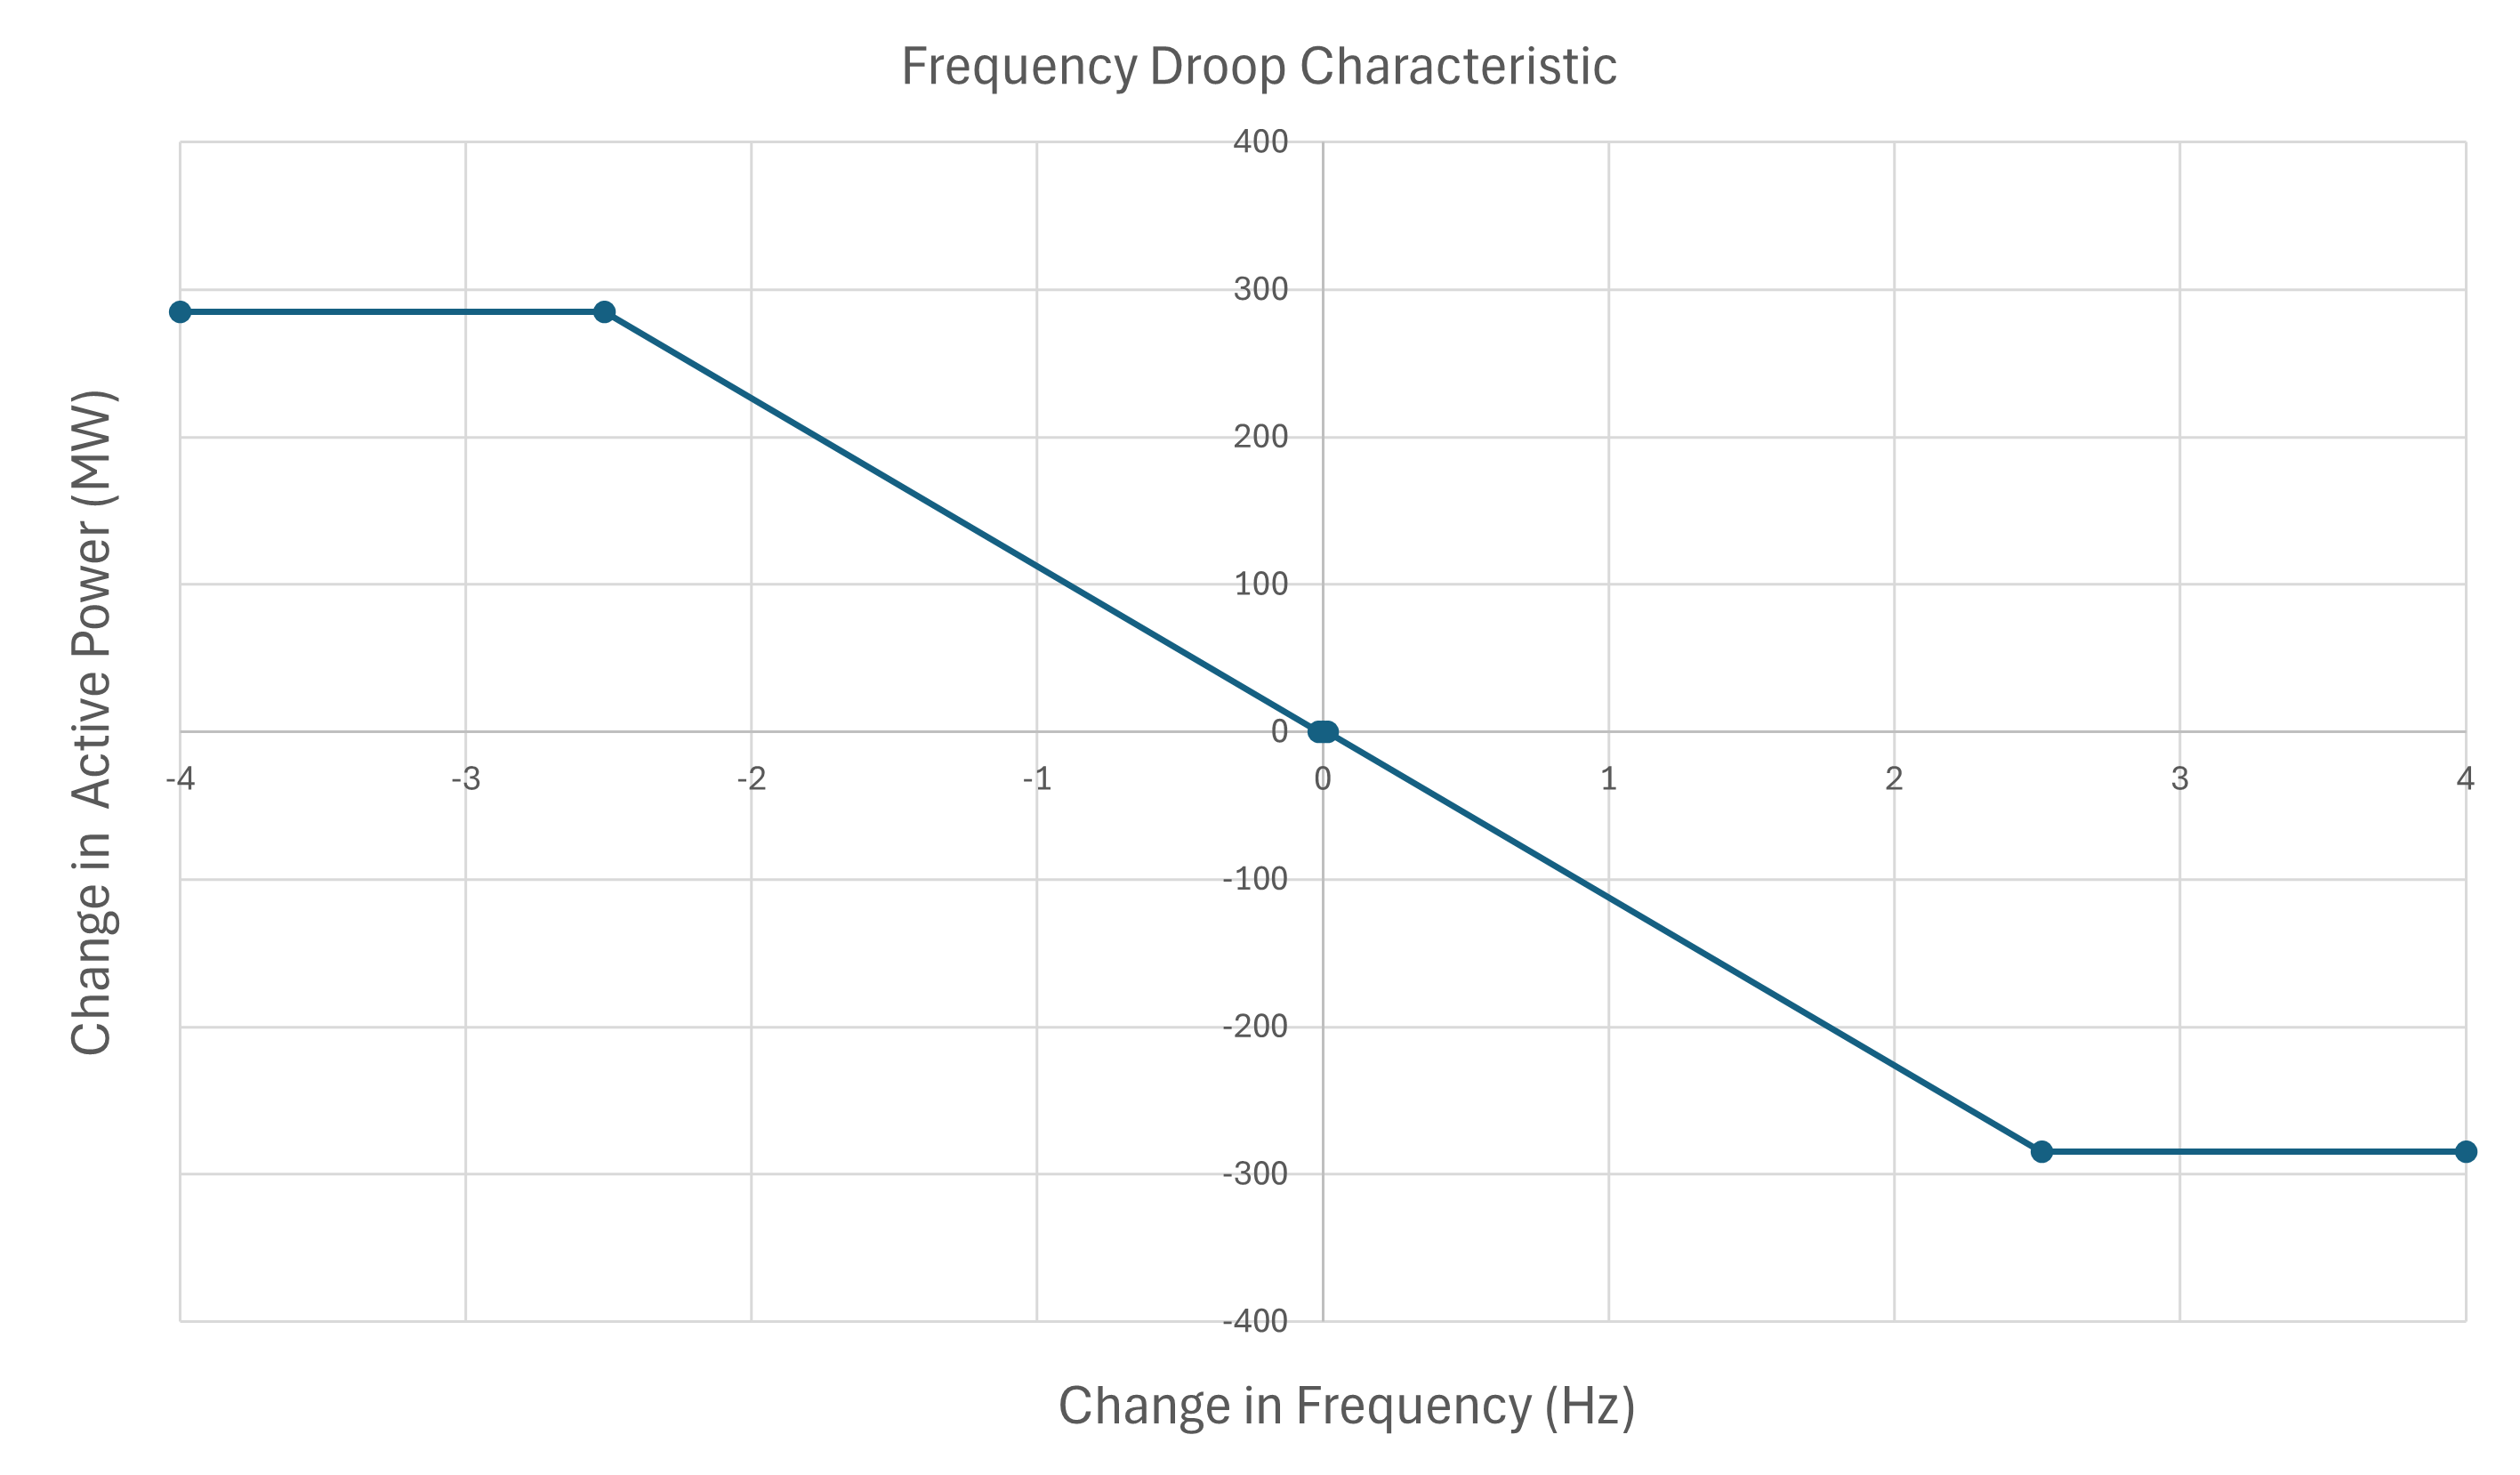
\includegraphics[width=0.9\textwidth]{report-assets/images/fdroop-char.png}
		\caption{Frequency droop characteristic}
		\label{fig:fdroop-char}
	\end{figure}
	
	\subsubsection{Frequency Droop Characteristics}
	
	
	Given the 5\% frerquency droop characteristic of the Heywood BESS, the corresponding relationship is defined as follows:
	

\[
\text{Droop=} \left[ \frac{\text{MW}}{\text{Hz}} \right] = \frac{1}{\Delta f / \Delta P} = \frac{\Delta P}{\Delta f} = \frac{P - P_{\text{set}}}{f - f_{\text{set}}}
\]



	
		{	
		\thicktablelines
		\begin{longtable}{|C{4cm}|C{4cm}|}%eg: {|C{5cm}|C{5cm}|}
			\caption{Frequency droop characteristic tabulated}%eg: {FRT parameters}
			\label{tab:frq-droop-char-new} \\% eg: {tab:frt-parameters} \\
			\toprule
			\rowcolor{tableheaderblue}
			\bfseries \color{white}Change in Frequency (Hz) & \bfseries \color{white}Active Power (MW) \\%eg: {\bfseries \color{white}Parameter & \bfseries \color{white}Unit & \bfseries \color{white}Value} \\
			\endhead
			\bottomrule \endfoot
			\csvreader[
			late after line=\\\hline,
			late after last line=,
			before reading={\catcode`\#=12},
			after reading={\catcode`\#=6}]% 
			{report-assets/frq-droop-char-new.csv}{}{\csvlinetotablerow} 
			\\\hline
		\end{longtable}
	}	
	
	\subsection{Fault ride through mode}
	
	Unlike a typical grid following plant, the grid forming BESS converters do not have a defined set of voltages at which they enter an FRT mode. The converters instead have a "virtual impedance" mode, which is activated following large voltage step change deviations at the converter terminals, which serves as its FRT mode. Under this mode, the plant injects current according to the reciprocal of a defined impedance, which acts as an equivalent to a "k-factor" commonly used in grid following FRT applications.

	Seperately to the converters, the plant PPC will freeze following point of connection voltages dropping below 0.85 or 1.15 p.u. The risk of PPC windup during FRT causing disturbances in operation is therefore mitigated.
	
	\section{Protection}
	
	The converters are equipped with frequency and voltage protection, which are set to keep the plant connected as per the NER requirements, but trip to avoid the plant supplying onto a faulted system. The frequency protection characteristic is shown in Figure \ref{fig:fprotection}. The voltage protection characteristic is shown in Figure \ref{fig:vprotection}.
	
	\begin{figure}[H]
		\centering
		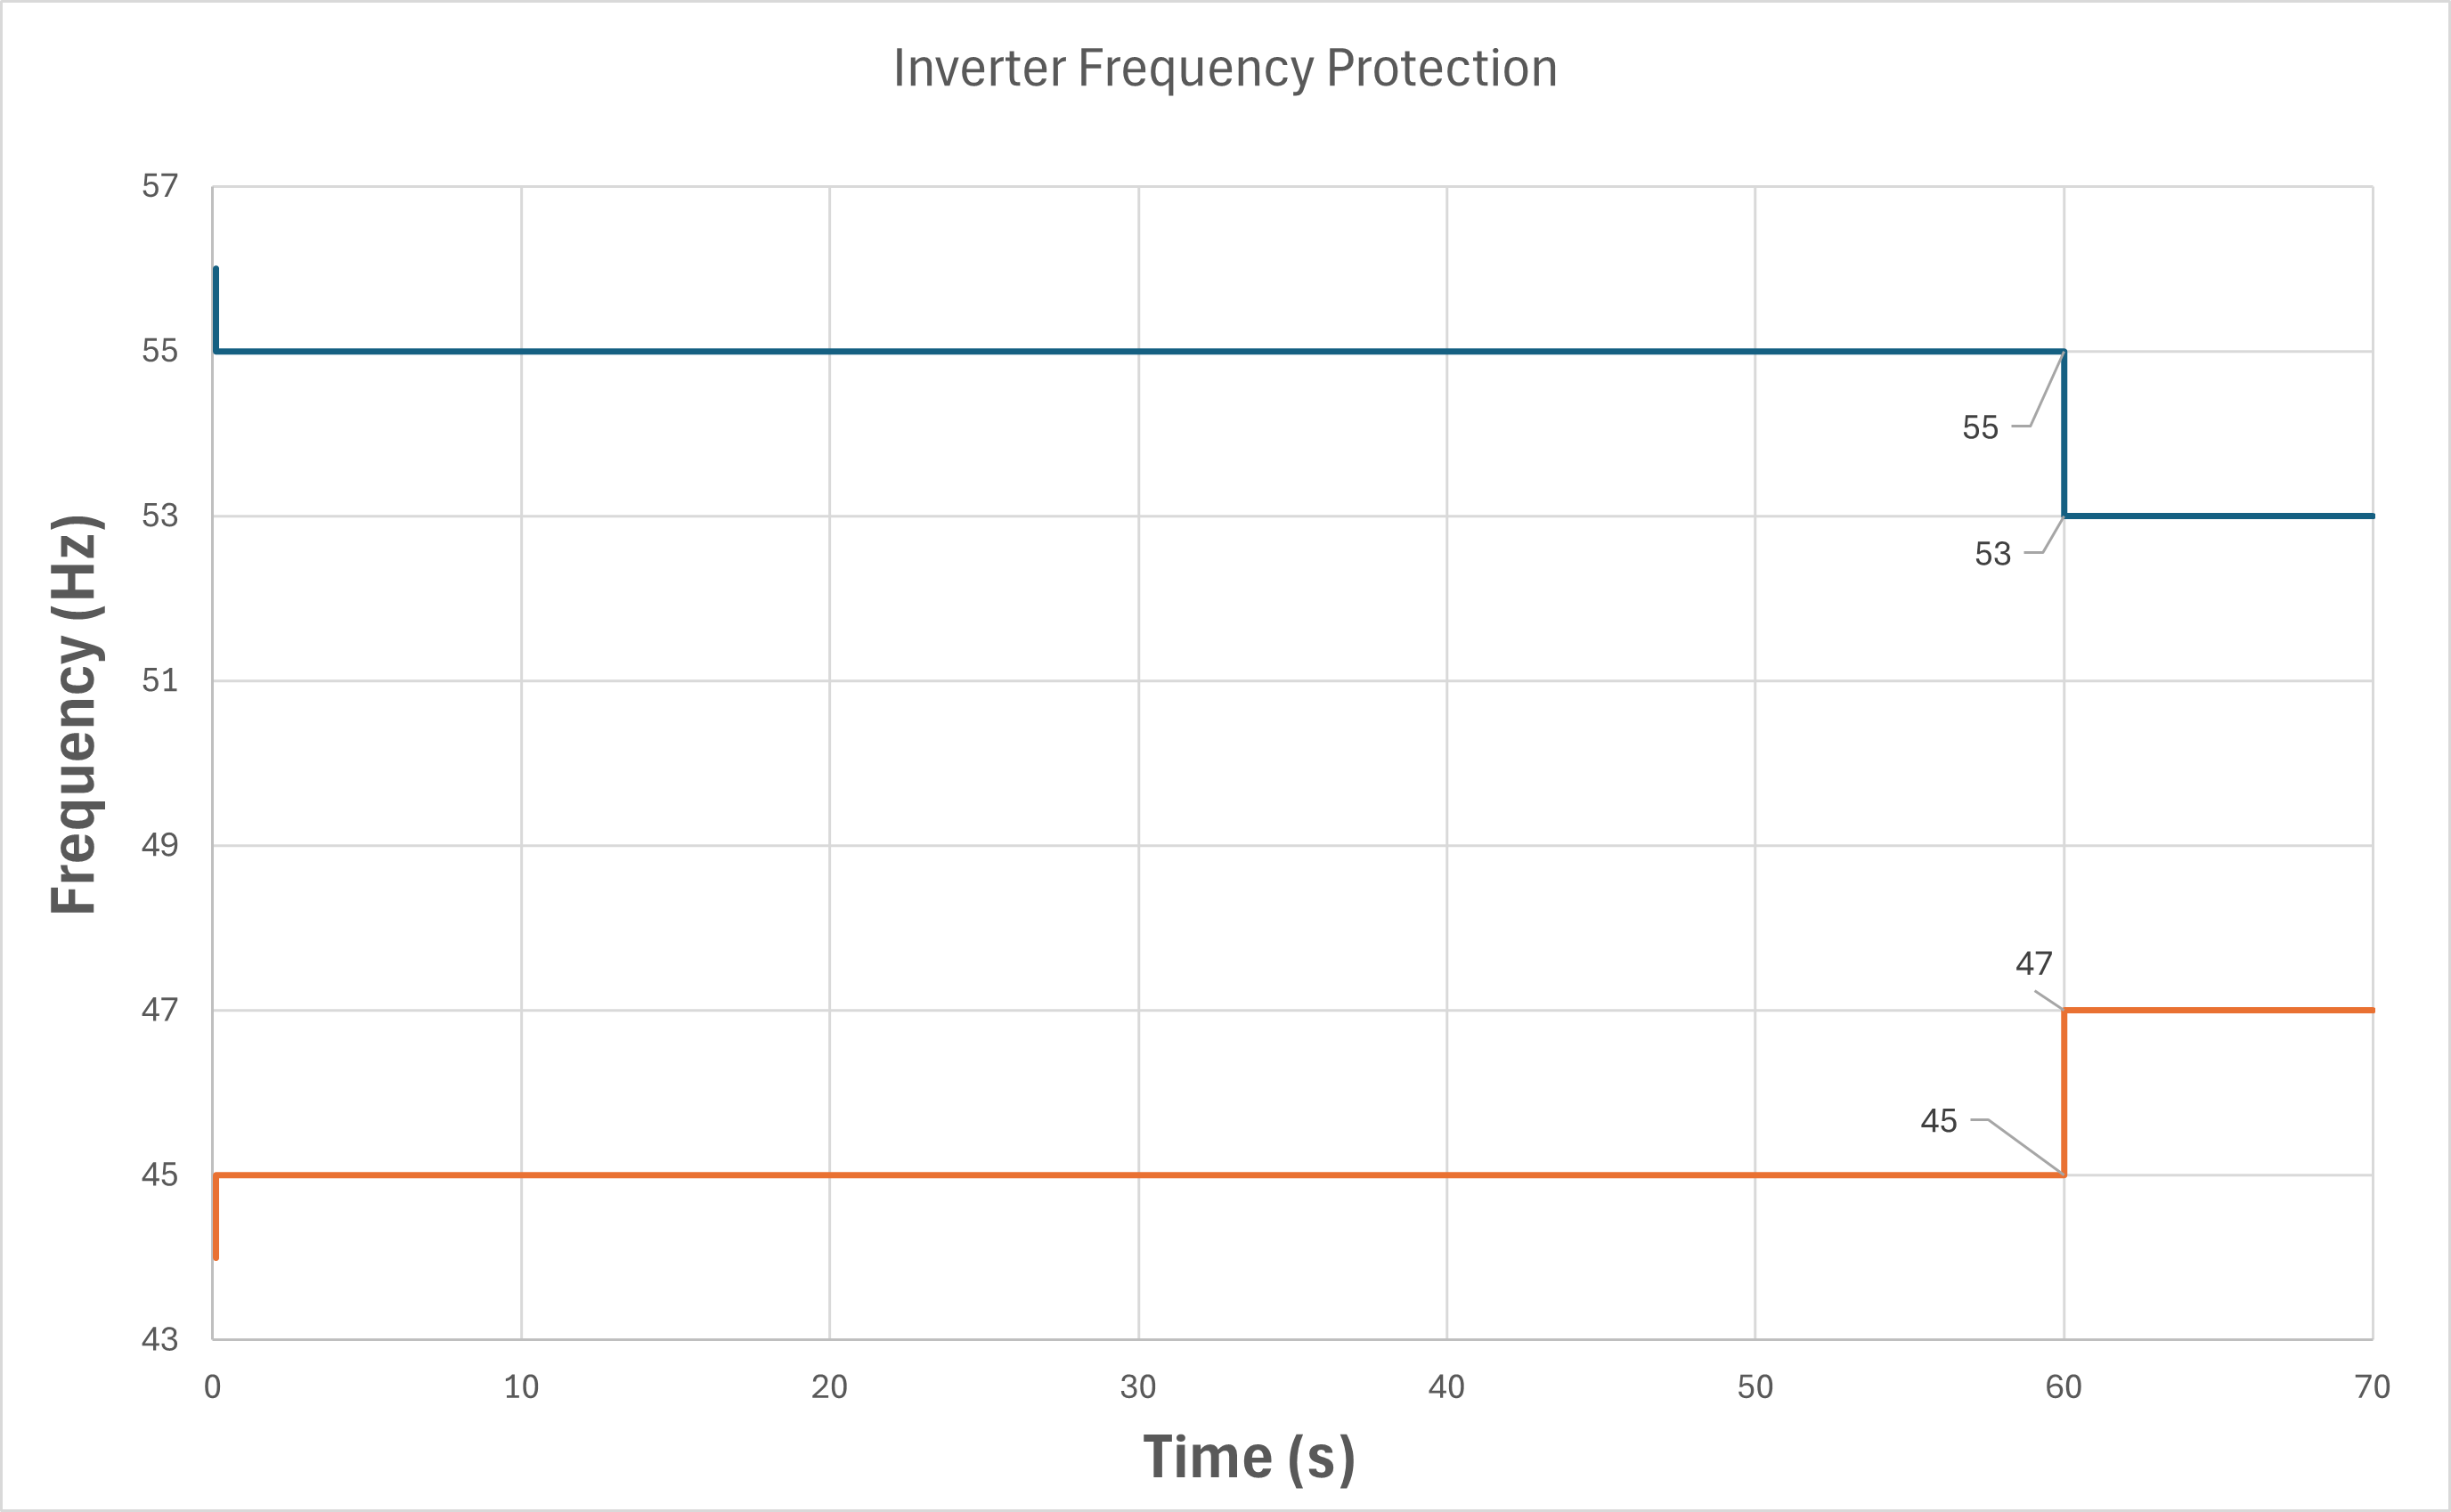
\includegraphics[width=0.6\textwidth]{report-assets/images/fprotection.png}
		\caption{Frequency protection characteristics}
		\label{fig:fprotection}
	\end{figure}
	
	\begin{figure}[H]
		\centering
		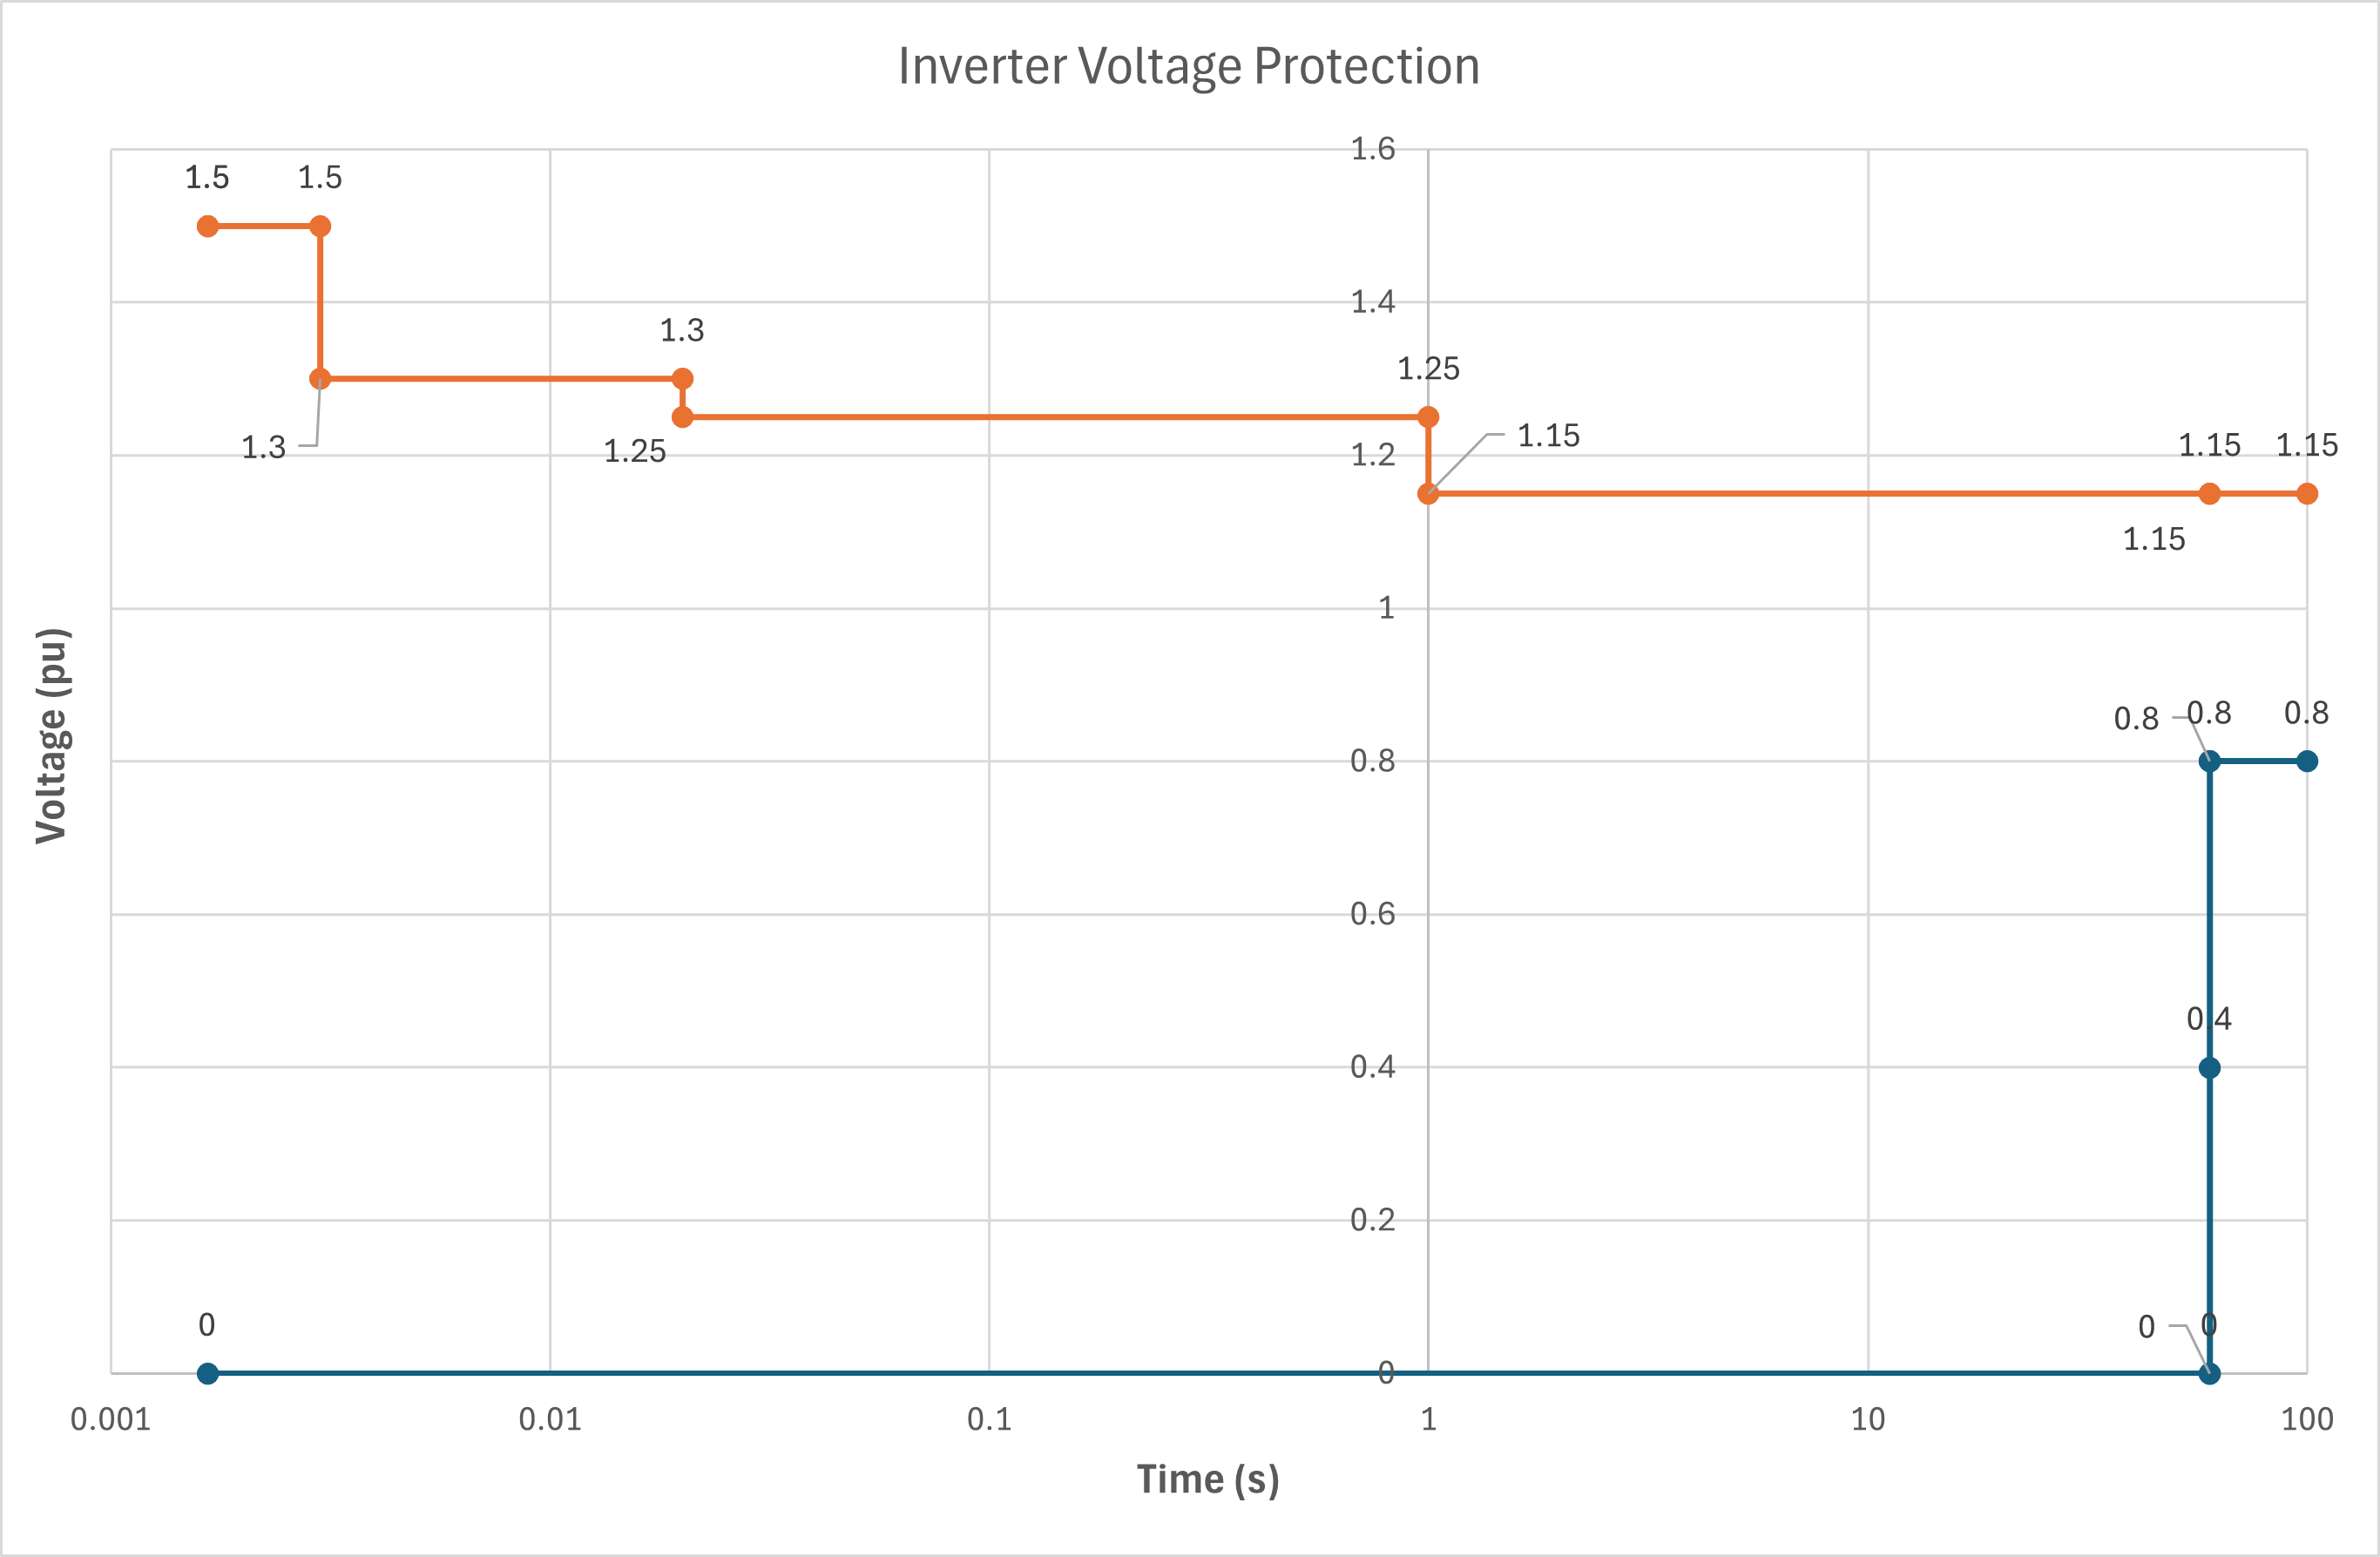
\includegraphics[width=0.6\textwidth]{report-assets/images/vprotection-new.png}
		\caption{Voltage protection characteristics}
		\label{fig:vprotection}
	\end{figure}

	\section{Simulation with a reduced number of converters}
	
	To perform simulations with a reduced number of converters on each branch,$n$, the following parameters need to be adjusted in the model
	
	\begin{itemize}
		\item Modify the Mbase of each aggregated converter to n x 4.6 MVA.
		\item Modify the Winding MVA of each aggregated converter transformer to n x 4.6 MVA.
		
	\end{itemize}
	
	All other parameters are in pu and will be adjusted automatically.
	
	\chapter*{Acronyms}
\begin{acronym}%[JSONP]\itemsep0pt
	\acro{AAS}{Automatic Access Standard}
	\acro{AEMO}{Australian Energy Market Operator}
	\acro{VSL}{Voltage Stackable Logic}
	\acro{AGC}{Automatic Generation Control}
	\acro{AVR}{Automatic Voltage Regulator}
	\acro{BESS}{Battery Energy Storage System}
	\acro{BOP}{Balance Of Plant}
	\acro{CGBESS}{Clements Gap BESS}
	\acro{Heywood BESS}{Heywood Battery Energy Storage System}	
	\acro{CSR}{Connection Studies Report}
	\acro{CT}{Current Transformer}
	\acro{CUO}{Continuous Uninterrupted Operation}
	\acro{HV}{High Voltage}
	\acro{DMAT}{Dynamic Model Acceptance Test}
	\acro{DYR}{PSSE Dynamics Data File}
	\acro{EMT}{Electromagnetic Transients}
	\acro{FIA}{Full Impact Assessment}
	\acro{FRT}{Fault Ride-Through}
	\acro{GPS}{Generator Performance Standards}
	\acro{HVRT}{High Voltage Ride-Through}
	\acro{LV}{Low Voltage}
	\acro{LVRT}{Low Voltage Ride-Through}
	\acro{MV}{Medium Voltage}
	\acro{NEM}{National Electricity Market}
	\acro{NSP}{Network Service Provider}
	\acro{OEM}{Original Equipment Manufacturer}
	\acro{OFRT}{Over-Frequency Ride-Through}
	\acro{OLTC}{On-Load Tap Changer}
	\acro{OPDMS}{Operations and Planning Data Management System}
	\acro{OVRT}{Over-Voltage Ride-Through}
	\acro{PLL}{Phase-Locked Loop}
	\acro{PLR}{Partial Load Rejection}
	\acro{PPC}{Power Plant Controller}
	\acro{PPM}{Power Plant Manager}
	\acro{RoCoF}{Rate of Change of Frequency}
	\acro{RMS}{Root Mean Square}
	\acro{RMU}{Ring Main Unit}
	\acro{RUG}{Releasable User Guide}
	\acro{S5251}{Reactive Power Capability}
	\acro{S5254}{Generating System Response to Voltage Disturbances}
	\acro{SCR}{Short Circuit Ratio}
	\acro{SMIB}{Single Machine, Infinite Bus}
	\acro{SLD}{Single Line Diagram}
	\acro{TOV}{Temporary Over-Voltage}
	\acro{UFRT}{Under-Frequency Ride-Through}
	\acro{UVRT}{Under-Voltage Ride-Through}
	\acro{VCS}{Voltage Control Strategy}
	\acro{WAN}{Wide Area Network}
	\acro{WF}{Wind Farm}
	\acro{VOIP}{Voice Over Internet Protocol}
	\acro{VRR}{Voltage Regulation Relay}
	\acro{VT}{Voltage Transformer}
\end{acronym}

	\chapter{Appendix A - PPC Model ICONs}
	

	%This is the start of the PPC paramters 
	\pgfplotstabletypeset[
	col sep=comma,            % Specifies the column separator in the CSV file
	string type,              % Allows string content in the table
	begin table=\begin{longtable},
		end table=\end{longtable},
	every head row/.style={   % Style for the header row
		before row=\toprule,  % Adds a top rule before the header
		after row=\midrule    % Adds a mid rule after the header
	},
	every last row/.style={   % Style for the last row
		after row=\bottomrule % Adds a bottom rule after the last row
	},
	columns/ICON/.style={column type=l},
	columns/Value/.style={column type=l},
	columns/Parameter/.style={column type=l},
	columns/Description/.style={
		column type={>{\RaggedRight\arraybackslash}p{13cm}}, % 5cm wide column with wrapping
	},
	]{report-assets/FLUENCEICONS.csv} % Path to your CSV file
	
	\chapter{Appendix B - PPC Model CONs}
    %This is the start of the PPC paramaters 
    

	\pgfplotstabletypeset[
	col sep=comma,            % Specifies the column separator in the CSV file
	string type,              % Allows string content in the table
	begin table=\begin{longtable},
	end table=\end{longtable},
	every head row/.style={   % Style for the header row
		before row=\toprule,  % Adds a top rule before the header
		after row=\midrule    % Adds a mid rule after the header
	},
	every last row/.style={   % Style for the last row
		after row=\bottomrule % Adds a bottom rule after the last row
	},
	 columns/Description/.style={
	column type={>{\RaggedRight\arraybackslash}p{13cm}}, % 5cm wide column with wrapping
	},
	]{report-assets/FLUENCE CONS.csv} % Path to your CSV file
   

		
	\chapter{Appendix C - PPC Model VARs}
	%This is the start of the PPC parameters
	\pgfplotstabletypeset[
	col sep=comma,            % Specifies the column separator in the CSV file
	string type,              % Allows string content in the table
	begin table=\begin{longtable},
		end table=\end{longtable},
	every head row/.style={   % Style for the header row
		before row=\toprule,  % Adds a top rule before the header
		after row=\midrule    % Adds a mid rule after the header
	},
	every last row/.style={   % Style for the last row
		after row=\bottomrule % Adds a bottom rule after the last row
	},
	columns/Description/.style={
		column type={>{\RaggedRight\arraybackslash}p{15cm}}, % 5cm wide column with wrapping
	},
	]{report-assets/FLUENCE VARS.csv} % Path to your CSV file

	\chapter{Appendix D - PPC Model STATEs}
	%This is the start of the PPC paramateres
	\pgfplotstabletypeset[
	col sep=comma,            % Specifies the column separator in the CSV file
	string type,              % Allows string content in the table
	begin table=\begin{longtable},
		end table=\end{longtable},
	every head row/.style={   % Style for the header row
		before row=\toprule,  % Adds a top rule before the header
		after row=\midrule    % Adds a mid rule after the header
	},
	every last row/.style={   % Style for the last row
		after row=\bottomrule % Adds a bottom rule after the last row
	},
	columns/Description/.style={
		column type={>{\RaggedRight\arraybackslash}p{15cm}}, % 5cm wide column with wrapping
	},
	]{report-assets/FLUENCE STATES.csv} % Path to your CSV file

	
	\chapter{Appendix E - Converter Model ICONs}
	
	%This is the start of the PPC paramateres
	\pgfplotstabletypeset[
	col sep=comma,            % Specifies the column separator in the CSV file
	string type,              % Allows string content in the table
	begin table=\begin{longtable},
		end table=\end{longtable},
	every head row/.style={   % Style for the header row
		before row=\toprule,  % Adds a top rule before the header
		after row=\midrule    % Adds a mid rule after the header
	},
	every last row/.style={   % Style for the last row
		after row=\bottomrule % Adds a bottom rule after the last row
	},
	columns/Description/.style={
		column type={>{\RaggedRight\arraybackslash}p{13cm}}, % 5cm wide column with wrapping
	},
	]{report-assets/SMAGF308ICONS.csv} % Path to your CSV file
	
	\chapter{Appendix F - Converter Model CONs}
	%this is the start of the converter parameters
	\pgfplotstabletypeset[
	col sep=comma,            % Specifies the column separator in the CSV file
	string type,              % Allows string content in the table
	begin table=\begin{longtable},
		end table=\end{longtable},
	every head row/.style={   % Style for the header row
		before row=\toprule,  % Adds a top rule before the header
		after row=\midrule    % Adds a mid rule after the header
	},
	every last row/.style={   % Style for the last row
		after row=\bottomrule % Adds a bottom rule after the last row
	},
	    columns/CON/.style={
		column type={>{\raggedright\arraybackslash}p{1cm}},
	},
	columns/Value/.style={
		column type={>{\raggedright\arraybackslash}p{2cm}},
	},
	columns/Parameter/.style={
		column type={>{\raggedright\arraybackslash}p{4.5cm}},
	},
	columns/Description/.style={
		column type={>{\RaggedRight\arraybackslash}p{10cm}}, % 5cm wide column with wrapping
	},
	]{report-assets/SMAGF308CONS.csv} % Path to your CSV file
	
	
	
	\chapter{Appendix G - Converter Model VARs}
	%This is the start of the converter parameters
	\pgfplotstabletypeset[
	col sep=comma,            % Specifies the column separator in the CSV file
	string type,              % Allows string content in the table
	begin table=\begin{longtable},
		end table=\end{longtable},
	every head row/.style={   % Style for the header row
		before row=\toprule,  % Adds a top rule before the header
		after row=\midrule    % Adds a mid rule after the header
	},
	every last row/.style={   % Style for the last row
		after row=\bottomrule % Adds a bottom rule after the last row
	},
	columns/Description/.style={
		column type={>{\RaggedRight\arraybackslash}p{10cm}}, % 5cm wide column with wrapping
	},
	]{report-assets/SMAGF308-VARS.csv} % Path to your CSV file
	
	\chapter{Appendix H - Extra Reactive Power Control Mode}	

	The following reactive power control modes are supported by Fluence functions but are not implemented in this project.
	\subsubsection{RPCM = 1 — Voltage Control Mode (VCMD)}	
	
	When RPCM is set to 1, the converter operates in voltage control mode, where reactive power is controlled to regulate the voltage at either a local or remote bus. Key parameters to adjust voltage control are shown below:
	
	\begin{itemize}
		\item ICON M+5 - must be set to 1 for the PPC to operate in voltage control mode
		\item VAR L+6 - can be adjusted to control the loca+l or remote bus voltage in pu
		\item ICON M+7 - can be set to 0 for local voltage or to a bus number for remote measurement
	\end{itemize} 
	
	\subsubsection{RPCM = 4 — Local Reactive Power Control Mode}

When RPCM is set to 4, the system enters local reactive power control mode. The reactive power command is provided directly by the user through VAR(L+2) (QLCLCMD). This mode can optionally be used with VSL enabled, by setting ICON(M+7) to 1, to allow the local Q reference to respond to bus voltage conditions. Key parameters to adjust reactive power control are shown below:

\begin{itemize}
	\item ICON M+5 - must be set to 4 for the PPC to operate in local reactive power control mode
	\item ICON M+7 - can be set to 1 for enabling the VSL function
	\item VAR L+2 - QLCLCMD can be adjusted to set the reactive power at the local branch
\end{itemize}

	\makebackpage
	
	
	
	
	
	
	
\end{document}